\section{Experiments}\label{sec:expts}

%Structure of this section?
% - Keep results and experiment protocols separate
% - But results can immediately follow the experiment protocols?
% - Datasets and higher-level research questions will be introduced up-front. 
% - Use sparse/noisy data motivation in the high-level research question to motivate use of UKPConvArgCrowdSample dataset.

% GPPL: M=500, P_m=10000

To evaluate our approach, we consider a number of different scenarios in which we test both classification performance, i.e. predicting binary pairwise labels, and ranking performance, i.e. predicting the order of preference of arguments.
We begin with a synthetic data experiment to illustrate how key methods work,
then evaluate the methods on real crowdsourced data for argumentation.
provided by \cite{habernal2016argument}, which was obtained using crowdsourcing.
The crowdsourced datasets contain pairwise preference labels for arguments taken from online discussion forums. 
Each pairwise label indicates "which argument is more convincing", or may express no preference.
We use four variants of this data, each of which involves different pre-processing steps.
All datasets contain 32 folds, which correspond to 16 controversial topics, and two stances for each topic.
The differences between the datasets are shown in Table \ref{tab:expt_data}.
\begin{table}
  \begin{tabularx}{\columnwidth}{ X }
  %Dataset %& Dataset properties \\%& Hypothesis & Methods \\
  \emph{UKPConvArgStrict} \newline 
  Combine crowdsourced labels with MACE and take $\ge 95\%$ most confident labels; \newline
  Discard arguments marked as equally convincing; \newline
  Discard conflicting preferences.
  %Bayesian method is competitive with previous methods at predicting clean preference pairs from a clean dataset. &
  %GP Preference learning + linguistic features + embeddings. 
  \\\hrulefill \\
  \emph{UKPConvArgAll} \newline
  Combine crowdsourced labels with MACE and take $\ge 95\%$ most confident labels; 
  %Bayesian method is competitive with previous methods if filtering step is removed. &
  %GP Preference learning + linguistic features + embeddings. 
  \\\hrulefill \\      
  \emph{UKPConvArgRank} \newline
  Combine crowdsourced labels with MACE and take $\ge 95\%$ most confident labels;  \newline
  PageRank used to produce ranking for each topic.
  %Bayesian method is competitive with previous methods at ranking arguments and 
  % can perform ranking given pairs rather than rank scores. &
  %GP regression with preference learning output + linguistic features + embeddings (trained on rank scores); \newline
  %GP Preference learning + linguistic features + embeddings (trained on pairs). 
  \\\hrulefill \\  
  \emph{UKPConvArgCrowdSample} \newline
  One original crowdsourced label per pair;\newline
  PageRank used to produce ranking for each topic. 
  %Bayesian method can predict argument pairs for individual annotators with competitive performance to rival methods on clean, combined data; \newline
  %There are patterns of common agreement/disagreement among workers. &
  %Bayesian Preference Components + linguistic features + embeddings (pair prediction). 
  %Bayesian model can predict individual argument rankings;\newline
  %Significant differences between individual rankings and gold-standard ranking. &
  %Bayesian Preference Components + linguistic features + embeddings (ranking output). 
  
  %UKPConvArgAll (train), UKPConvArgStrict (test) &
  %Use the original pairs for training and try to predict the cleaned output &
  %(Optional -- more about preference learning from noisy data, so probably deserves a separate paper/student project?)
  %Show that the model can also be used to predict a gold standard -- end-to-end preference learning &
  %Bayesian Preference Components + linguistic features + embeddings + gold-standard pairs on the training data (model is not really designed for aggregation, but for sharing information between similar people and items; without gold standard training labels, we need to know the y-feature mixture of the gold-standard); 
  %HeatmapBCC with preference learning forward model (deals directly with noisy labels, rather than different opinions about convincingness; useful for learning from implicit feedback)
  \end{tabularx}
  \caption{\label{tab:expt_data} Summary of the processing steps used to produced the gold-standard data for each fold in each different dataset.}
\end{table}

A major aim of our experiments is to compare our Bayesian preference learning method,
which we refer to here as \emph{GPPL},
against the \emph{SVM} and \emph{BLSTM} methods used in \cite{habernal2016argument}. For classifications, 
SVM and BLSTM concatenates the feature vectors of each pair of arguments. 
For ranking, SVM and BLSTM are used to perform regression and are trained on the output of the PageRank 
model run over items in the training folds.
As well as comparing classification and ranking performance, 
we also investigate how each method resolves conflicting preference pairs in crowdsourced data;
which types of input features are useful for modelling convincingness;
how well each method estimates uncertainty and how well it performs with active learning to address cold-start problems; and how well does each method cope with data sparsity, e.g. in a cold-start situation,
 and noisy data.

\subsection{Experiment 1: Toy Data}

Our two tasks are to \emph{score} arguments in terms of convincingness and to 
\emph{classify} the preference label for a pair of arguments, i.e. predict which of the arguments will be preferred. 
We use simulated data to show how Gaussian process preference learning
differs from the established approaches for each task, namely SVM for 
the classification task and PageRank for the scoring task.
Our simulation consists of four scenarios; 
in each scenario, we assume a set of pairwise preference labels for arguments labelled
arg0 to arg4.  
The pairwise labels are depicted as convincingness graphs in Figure \ref{fig:arg_graphs}.
Arrows indicate the     
preferred arguments, e.g. the first plot shows that arg3 is more convincing than arg4. 
Each scenario is repeated 25 times and in each run we select arguments at random from one fold of the UKPConvArgStrict, 
then associate these arguments with the labels arg0 to arg4.  
For each argument, we obtain a feature vector by computing mean Glove word embeddings as in \cite{habernal2016argument}.
We trained PageRank, GPPL and the SVM classifier on the preference pairs shown in each graph. The PageRank scores and GPPL latent preference function means for each argument are shown in Figure \ref{fig:scores}. The first scenario, "no cycle" shows a simple dataset where
arg0 is preferred to both arg1 and arg2, which is reflected in both the PageRank and GPPL scores in Figure \ref{fig:scores}. However, arg3 and arg4 are not connected to the rest of the graph and receive different scores with PageRank and GPPL. 
The classifications for pairs of arguments produced by GPPL and SVM are shown in 
Figures \ref{fig:gppl_classifications} and \ref{fig:svm_classifications}.
GPPL provides probabilistic classifications that give less confident estimates for many
of the pairs that were not yet observed, e.g. 2 $\succ$ 4.

The second scenario, "single cycle", shows how each method handles a cycle in the preference graph.
Both PageRank and GPPL produce even values for the arguments in the cycle (arg0, arg1 and arg2). PageRank assigns lower scores to both arguments that are not in the cycle (arg3 and arg4), while GPPL gives a higher score only to the preferred argument, arg3. The 
SVM predictions for  "single cycle" predict that arg0 and arg1 are preferred over arg3,
although arg0 and arg1 are in a cycle and it is unclear why arg0 and arg1 would be preferred. GPPL in contrast gives a weak prediction that arg3 is preferred.

The third scenario, "double cycle" produces very different results with PageRank and GPPL. Here, the argument graph shows two paths from arg2 to arg0 via arg1 or arg3, and one conflicting
preference arg2 $\succ$ arg0. GPPL scores the arguments as if the single conflicting preference, arg2 $\succ$ arg0, was not present, likely giving more weight to two parallel paths from arg2 to arg0. 
In contrast, PageRank gives high scores to both arg0 and arg2.
The classifications by GPPL and SVM are similar, but GPPL produces more uncertain 
predictions than in the first scenario, likely due to the conflicting edge.

Finally, "cycle with 9 undecided prefs" shows an exaggerated scenario in which
we have added nine "undecided" preference labels to the "no cycle" scenario.
The undirected edges indicate that neither argument was preferred and simulate the
case where multiple annotators were asked to label a pair and did not all agree. 
This does
not affect the PageRank scores, but reduces the difference in GPPL scores between arg0 and other arguments, since the preference arg2 $\succ$ arg0 is
effectively given less weight due to the undecided labels. This is reflected in the 
predicted classifications from GPPL, which are less confident than in the "no cycle" scenario.
The SVM cannot be trained using the uncertain labels and therefore does not adapt to the undecided labels. 

In conclusion, GPPL appears to resolve conflicts in the preference graphs in a
more intuitive manner than PageRank, which was designed for ranking web pages by 
importance and therefore may be less suitable for ranking by preference. In contrast
to SVM, it is able to account for undecided labels to soften the underlying convincingness function.
\begin{figure*}
% We also have the "single_hub" experiment but excluded because it is too trivial. The interesting result there
% is that SVM_probas are overly confident; we can also see that effect in "undecided".
\subfloat[Argument preference graphs for each scenario.]{
\label{fig:arg_graphs}
\addtocounter{subfigure}{-4}
\captionsetup[subfigure]{labelformat=empty}
\subfloat[no cycle]{
  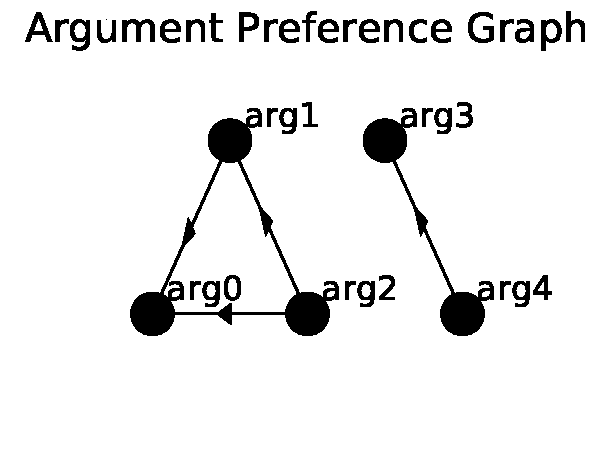
\includegraphics[width=0.5\columnwidth, clip=True, trim=30 30 20 30]{figures/cycles_demo/no_cycle/arggraph_arg_graph}
}
\subfloat[single cycle]{
  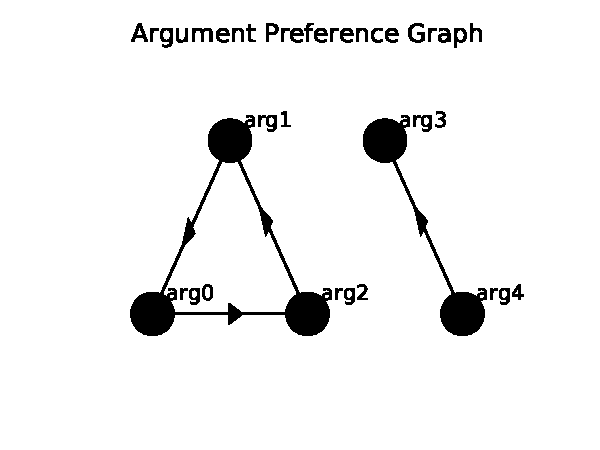
\includegraphics[width=0.5\columnwidth, clip=True, trim=30 30 20 30]{figures/cycles_demo/simple_cycle/arggraph_arg_graph}
}
\subfloat[double cycle]{
  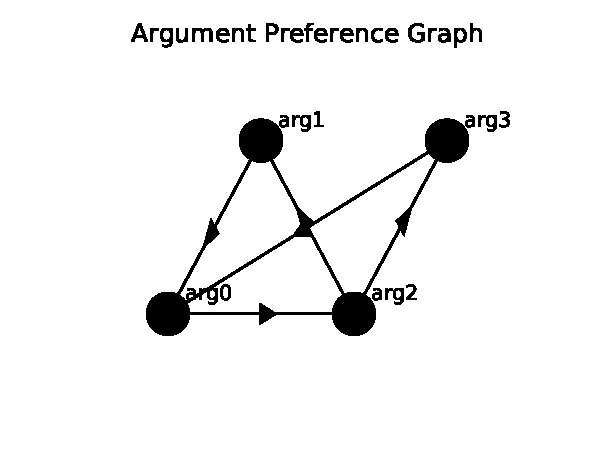
\includegraphics[width=0.5\columnwidth, clip=True, trim=30 30 20 30]{figures/cycles_demo/double_cycle/arggraph_arg_graph}
}
\subfloat[cycle with 9 undecided prefs.]{
  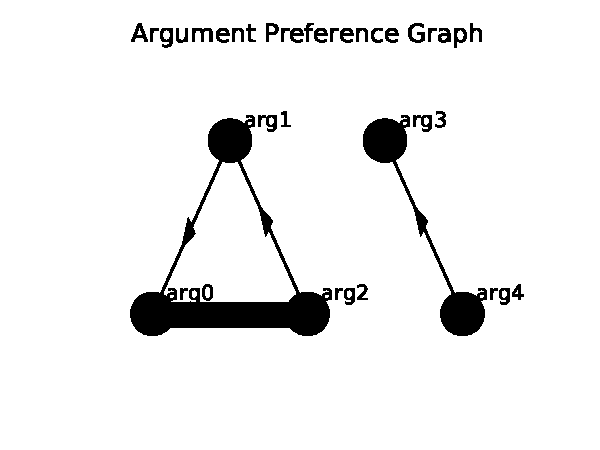
\includegraphics[width=0.5\columnwidth, clip=True, trim=30 30 20 30]{figures/cycles_demo/undecided/arggraph_arg_graph}
}
}\\
\subfloat[Ranking scores for arguments (bars for GPPL show standard deviation of latent preference function)]{ 
\label{fig:scores}
  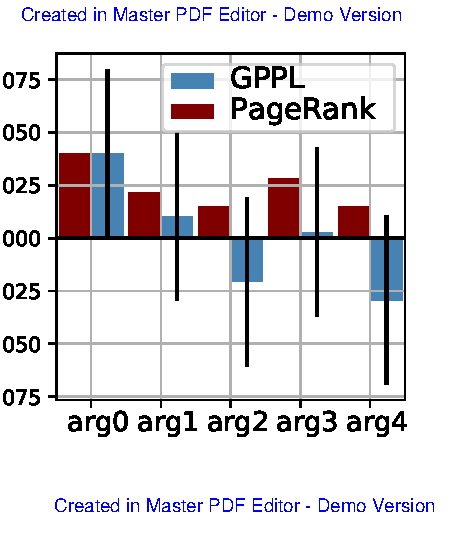
\includegraphics[width=0.5\columnwidth, clip=True, trim=20 5 10 22]{figures/cycles_demo/no_cycle/PageRank_scores}
%}
%\subfloat[]{ 
  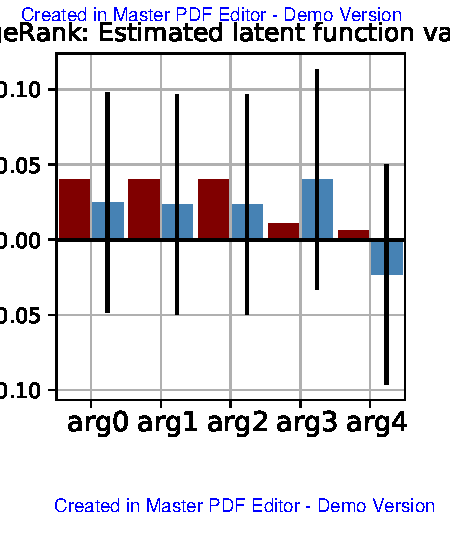
\includegraphics[width=0.5\columnwidth, clip=True, trim=20 5 10 22]{figures/cycles_demo/simple_cycle/PageRank_scores}
%}
%\subfloat[]{ 
  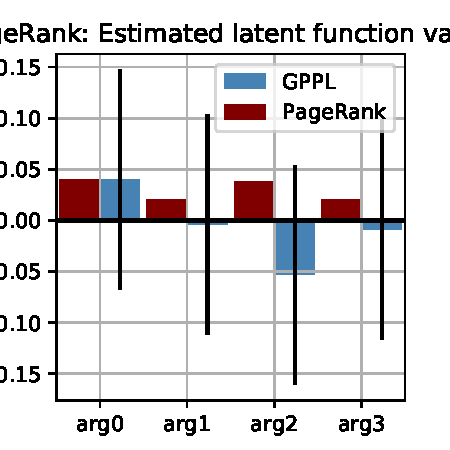
\includegraphics[width=0.5\columnwidth, clip=True, trim=20 5 10 22]{figures/cycles_demo/double_cycle/PageRank_scores}
%}
%\subfloat[]{ 
  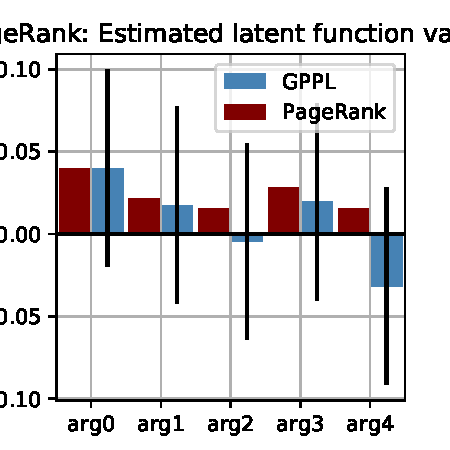
\includegraphics[width=0.5\columnwidth, clip=True, trim=20 5 10 22]{figures/cycles_demo/undecided/PageRank_scores}
}\\
\subfloat[GPPL predictions: probability that the argument 
on the horizontal axis is preferred to the argument on the vertical axis.]{
\label{fig:gppl_classifications}
  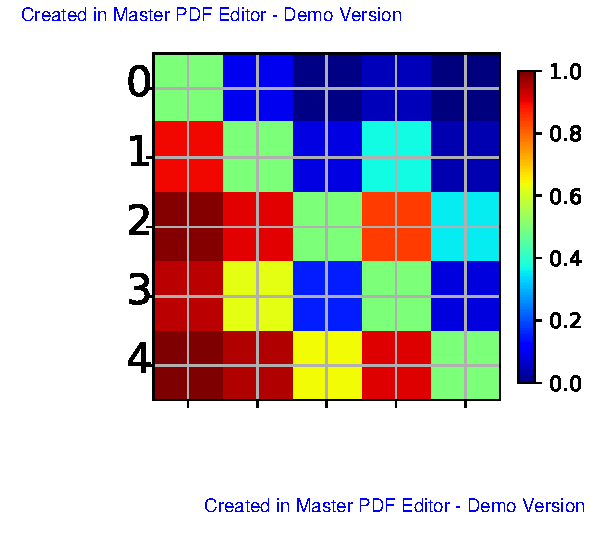
\includegraphics[width=0.49\columnwidth, clip=True, trim=58 5 41 24]{figures/cycles_demo/no_cycle/GPPL_probas}
%}
%\subfloat[]{
  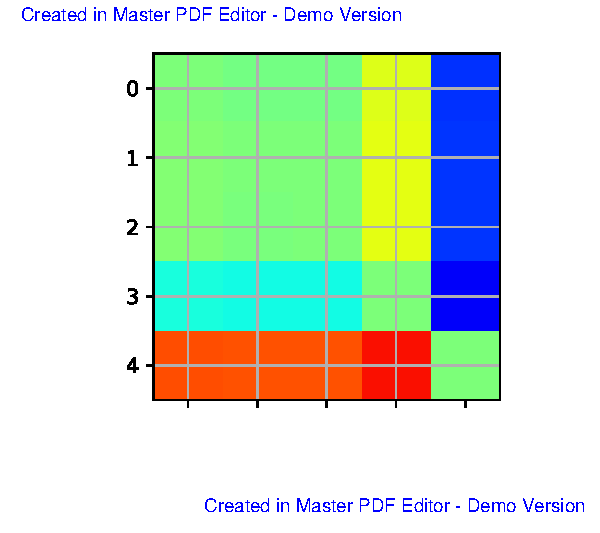
\includegraphics[width=0.49\columnwidth, clip=True, trim=58 5 41 24]{figures/cycles_demo/simple_cycle/GPPL_probas}
%}
%\subfloat[]{
  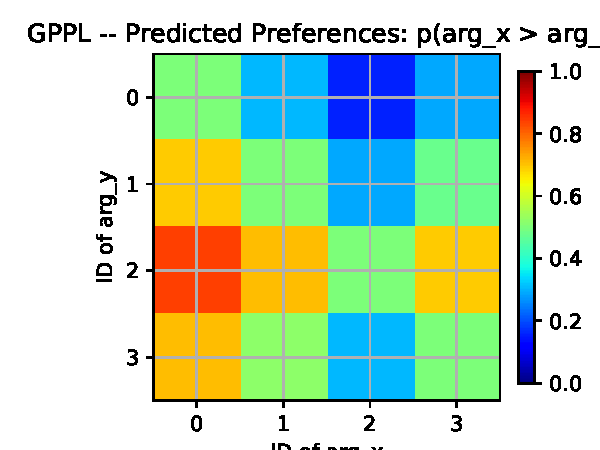
\includegraphics[width=0.49\columnwidth, clip=True, trim=58 5 41 24]{figures/cycles_demo/double_cycle/GPPL_probas}
%}
%\subfloat[]{
  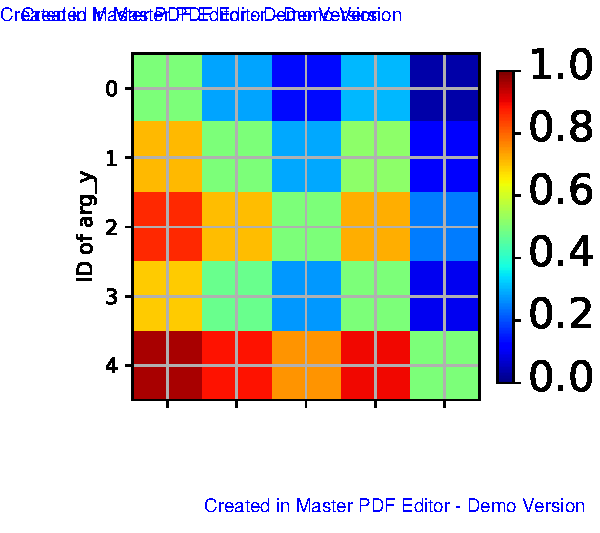
\includegraphics[width=0.56\columnwidth, clip=True, trim=58 5 10 24]{figures/cycles_demo/undecided/GPPL_probas}
}\\
\subfloat[SVM predictions: probability that the argument 
on the horizontal axis is preferred to the argument on the vertical axis.]{
\label{fig:svm_classifications}
  \includegraphics[width=0.49\columnwidth, clip=True, trim=58 5 41 24]{figures/cycles_demo/no_cycle/SVM_probas} 
%}
%\subfloat[]{
  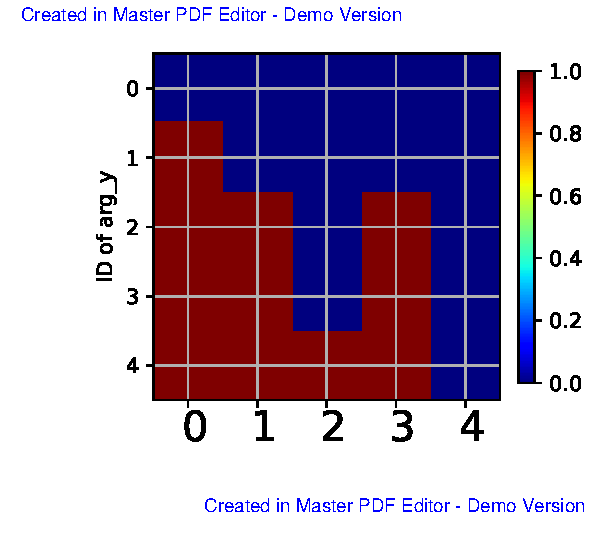
\includegraphics[width=0.49\columnwidth, clip=True, trim=58 5 41 24]{figures/cycles_demo/simple_cycle/SVM_probas} 
%}
%\subfloat[]{
  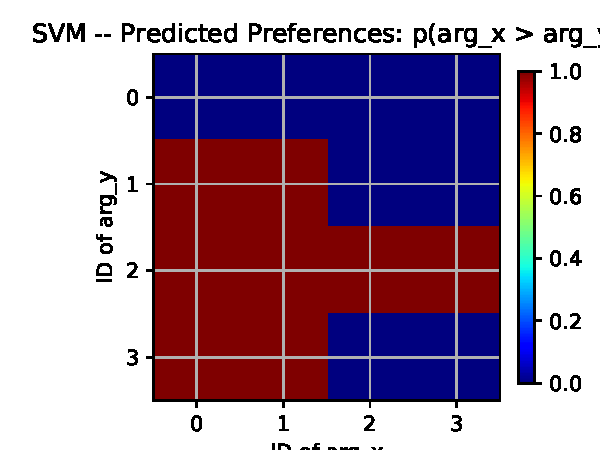
\includegraphics[width=0.49\columnwidth, clip=True, trim=58 5 41 24]{figures/cycles_demo/double_cycle/SVM_probas} 
%}
%\subfloat[]{
  \includegraphics[width=0.56\columnwidth, clip=True, trim=58 5 10 24]{figures/cycles_demo/undecided/SVM_probas} 
}
\caption{Preference graphs and predictions for simulated arguments in different scenarios. The plots in each column correspond to a single scenario.}
\end{figure*}

\subsection{Experiment 2: Clean Data}

We first compare GPPL to the SVM and BLSTM methods for classification on the UKPConvArgStrict dataset and ranking on the UKPConvArgRank dataset. Both datasets were
cleaned to remove disagreements between annotators.
We compared GPPL with different sets of input features with the length-scale set using the median heuristic: first, we use ~32000 linguistic features (labelled as \emph{ling})
that we also use for the SVM (as in \cite{habernal2016argument}), second, the Glove 
word embeddings with 300 dimensions that we also use for the BLSTM (also as in \cite{habernal2016argument},
labelled \emph{Glove}),
and finally, the combination of both linguistic features and embeddings (labelled \emph{ling + Glove}). 
To create embeddings for an argument, we take the mean of the individual word embeddings for the tokens in the argument.

We also compare multiplicative and additive combinations for the kernel functions and
test three different settings for the hyper-parameters $a_0$ and $b_0$, which control
the noise variance. While it may be possible to further optimise $a_0$ and $b_0$,
we found weak priors favouring a moderate level of noise to be most
effective and therefore continue to use $a_0=2$, $b_0=200$ in the remaining experiments.
We also tested $a_0=1$, $b_0=1$, which favours lower noise variance, but this resulted in
a cross entropy error (CEE) of $0.69$ because the predicted classifications were very close to $0.5$, compared to CEE of $0.47$ when using $a_0=2$, $b_0=200$. With stronger
priors $a_0=2e3$, $b_0=2e5$, we observed a drop in accuracy of $7\%$ on UKPConvArgStrict so concluded that $a_0=2$, $b_0=200$ is a reasonable setting to proceed without further optimisation.

%\begin{enumerate}
%  \item Which type of kernel combination is most effective for GPPL? We compare with both heuristic length-scale and optimized, in case the heuristic is poor for one of the kernel combinations. Result: little difference between additive and multiplicative kernels over the features. GP methods are heavily affected by choice of kernel. The standard approach (using a product of kernels for each feature) is equivalent to taking the euclidean distance between points in feature space. These distances become very large when we have a large number of features. Each point needs to be close in all dimensions in order to be close overall. An alternative to this product kernel is to use a sum kernel, which will result in points having strong covariance if some (rather than all) features are similar. This may be suitable for high-dimensional settings where some features may have missing values. Compare the GPPL approach with product and sum kernels. 
%  \item Besides the choice of kernel itself, another important set of hyperparameters of the GPPL are the hyperparameters for the prior over the output scale of the kernel. The output scale controls the noise of the preferences, and needs to be large enough to allow the posterior to deviate substantially from the prior mean given only a small number of observations at each point. We test three different plausible settings of this hyperparameter to determine how sensitive the results are. Result: heavily informative values do not work well; very noninformative values are effective, although we observe a small boost when using an intermediate setting. This may be due to the data sparsity; the intermediate setting puts more weight onto each individual observation.
%\end{enumerate}

%% IMportant results have been merged into 2
%\begin{table}
%  \begin{tabularx}{\columnwidth}{ | l | X |  X |  X |  X | X| X|} \hline
%\multicolumn{7}{| l |}{UKPConvArgStrict} \\   \hline
% & \multicolumn{4}{|l|}{median heuristic} & \multicolumn{2}{|l|}{ARD} \\ 
%Kernel: & + & \multicolumn{3}{ l |}{*} & + & *\\ 
%$a_0$:  & 2    & 2    & 1    & 2e3 & 2 & 2\\ \hline
%$b_0$:  & 200  & 200  & 1    & 2e5 & 200 & 200 \\ \hline
%\\ \hline
%Acc.:   & 0.78 & 0.79 & 0.80 & 0.72  & ? & 0.80\\
%AUC:    & 0.86 & 0.87 & 0.87 & 0.79 & ? & 0.87 \\
%CEE:    & 0.69 & 0.47 & 0.69 & 0.39 & ?  & 0.51 \\
%\hline \multicolumn{7}{| l |}{UKPConvArgRank} \\   \hline
%Pears.: & 0.40 & 0.45 & 0.43 & - & ?  & 0.44 \\
%Spear.: & 0.64 & 0.65 & 0.67 & - & ? & 0.67 \\
%Kend.:  & 0.49 & 0.49 & 0.50 & - & ? & 0.50 \\
%\hline
%  \end{tabularx}
%  \caption{Different hyper-parameters and kernel combinations for 
%  GPPL with Glove + ling features}
%\end{table}

The results are shown in Table \ref{tab:clean_results}. When using \emph{ling} features,
GPPL produces similar accuracy and improves the area under the ROC curve (AUC) by 2\%,
and cross entropy error by 0.01. Much larger improvements can be seen in the ranking metrics. When GPPL is run with mean Glove embeddings, it performs worse than
BLSTM for classification but improves the ranking metrics. Using a combination of features,
GPPL performs substantially better than the alternative methods for both classification and
ranking, suggesting that embeddings and linguistic features contain complementary information.

We also apply the MLII optimisation method to GPPL with \emph{ling+Glove} features. The results are labelled as "OptGPPL" in Table \ref{tab:clean_results}, and show that 
optimising the length-scale using Bayesian model selection can further improve performance
above the median heuristic. However, the cost of these improvements is that each fold required around 2 hours to compute instead of approximately 10 minutes on the same machine (an Intel i7 quad core desktop) using the median heuristic. The accuracy for each fold with and without length-scale optimisation is shown in 
Table \ref{tab:opt_by_fold}, and shows that optimisation does not always improve performance. 
Since the optimisation step is performed using only the training folds and the test is performed 
on a different topic, there is a possibility of overfitting: features that are important in the 
test fold may not appear relevant in the training folds. 
Optimisation may therefore be more effective if it could be 
executed in a semi-supervised manner by including unlabelled data from the target topic.

We hypothesise that GPPL benefits from a Bayesian approach that integrates learning from
discrete preference labels with regression over a latent preference function. To test this,
we compare GPPL against a two stage method: first, we use use the GPPL preference likelihood method without any item features to infer convincingness scores for each argument from the pairwise labels; second, we perform SVM regression trained on the inferred scores with \emph{ling+Glove} features.
Hence we investigate whether the benefits of GPPL are entirely due its different preference likelihood in contrast to training the SVM classifier directly or using PageRank to estimate scores.
 The results are shown in Table \ref{tab:clean_results} as \emph{PL+SVR}, 
 and show that while this approach does not reach the same performance as 
 GPPL. This may be due to the benefits of integrating a GP to map the features to the latent
 function, rather than using a separate SVM regressor.
 
For the pairwise classification task, we also compare GPPL against a Gaussian process classifier (\emph{GPC}) to investigate whether other GP-based approaches produce comparable performance. As shown in Table \ref{tab:clean_results}, GPC produces the best results on the classification task, although it cannot be used
to rank the arguments.
While the classification approach involves learning over twice as many features -- the features of the first and second items in each pair are concatenated -- the GPC may perform better on this dataset 
because it is trained directly on the classification task, rather than through a preference learning likelihood. 
% However, while this demonstrates some benefits of GP approach, the GPC cannot readily be used for ranking arguments.

%\begin{enumerate}
%  \item Compare GP preference learning (GPPL) to SVM using linguistic features. Result: better performance on ranking tasks.
%  \item Compare GPPL to Bi-LSTM. Result: GPPL is not as effective with mean embeddings, but GPPL with linguistic features still outperforms Bi-LSTM on all metrics.
%  \item Do the embeddings and linguistic features provide complementary information? Run GPPL with both sets of features. Result: improvement on classification tasks; larger improvement on ranking; suggests that the feature sets contain complementary information. The computational cost (of kernel computation, which dominates the overall cost in these experiments) grows linearly with number of features.
%  \item Does GPPL improve ranking performance because of the preference likelihood, or the way it makes predictions? Compare against feature-free preference learning used to train an SVM regression model (PL+SVR). Result: GPPL improves classification slightly on noise-free dataset, and improves more over PL+SVR on ranking and noisy classification tasks. GPPL resolves conflicts at the same time as predicting scores using similarities between arguments in feature space, so therefore has more information to resolve erroneous labels than the feature-free PL.
%  \item Performance improvements may be down to using a Bayesian approach with sparse data. Can we improve 
%  classification performance by training a GP Classifier rather than using GPPL? The feature space is increased by 
%doing this. Result: improvements on strict dataset but not when there is more noise. Maybe a downside of increased 
%sparsity meaning that erroneous points are further away from any correct points that would resolve the problems? 
%  \item What is the benefit of length-scale optimisation for GPPL versus our heuristic length-scale estimates? 
%Result: there is a performance improvement but it is not completely consistent (can overfit) and it comes at a 
%large cost. Therefore, our other comparisons will use the heuristic length-scales unless stated.  
%\end{enumerate}

\begin{table*}
  \begin{tabularx}{\textwidth}{ | l  | X |  X |  X |  X |  X | X | X | X | X | X |}
  \hline
\multicolumn{11}{| l |}{UKPConvArgStrict} \\   \hline
       &SVM  &BLSTM&\multicolumn{3}{c|}{GPPL*, medi.}&GPPL*, opt & GPPL+, medi. & GPPL+, opt & PL +SVR    & GPC \\\hline
       &ling &Glove  &ling &Glove &\multicolumn{6}{c|}{ling+ Glove}\\\hline
Acc.:  &0.78 &0.76   &0.78 &0.71  &0.79  & 0.80  & 0.78 & 0.78  & 0.78  & 0.81 \\
AUC:  &0.83 &0.84   &0.85 &0.77  &0.87  & 0.87 & 0.86  &  0.86 & 0.85  & 0.89 \\
CEE:   & 0.52 &0.64  &0.51 &1.12  &0.47  & 0.51 & 0.69  & 0.69 & 0.51  & 0.43 \\
\hline \multicolumn{11}{| l |}{UKPConvArgRank} \\   \hline
Pears.:&0.36&0.32   &0.38 &0.33  &0.45  &  0.44 & 0.40 &  0.40 & 0.39  & - \\
Spear.:&0.47&0.37   &0.62 &0.44  &0.65  &  0.67 & 0.64 &  0.64 & 0.63  & - \\
Kend.: &0.34&0.27&0.47 &0.31  &0.49     &  0.50 & 0.49 &  0.49 & 0.47  & - \\
\hline
  \end{tabularx}
  \caption{Performance comparison on clean datasets. }
  \label{tab:clean_results}
\end{table*}

\begin{table}
\npdecimalsign{.}
\nprounddigits{2}
\npnoaddmissingzero
  \begin{tabularx}{\columnwidth}{ p{3.2cm}  | p{1.7cm} | n{0}{2} | n{0}{2} }
 Topic & Stance & {M.H.} & {Opt.} \\
\hline\hline
\multirow{ 2}{*}{\parbox{ 3.2cm}{Ban plastic water bottles?}} & no & .8125 & .80902778\\
& yes & .83 & .8825 \\ \hline

\multirow{ 2}{*}{\parbox{ 3.2cm}{Christianity or atheism?}} & atheism & .82874618 & .81345566\\
 & Christianity & .78076923 & .76923077\\ \hline

\multirow{ 2}{*}{\parbox{ 3.2cm}{Evolution vs creation}} & creation & .86516854 & .88764045\\
& evolution & .72941176 & .72\\ \hline

\multirow{ 2}{*}{\parbox{ 3.2cm}{Firefox vs Internet Explorer}} & IE & .8649635  & .83576642\\
& firefox & .86708861 & .85864979\\ \hline

\multirow{ 2}{*}{\parbox{ 3.2cm}{Gay marriage -- right or wrong?}} & right & .77722772 & .76237624\\
& wrong & .86353468 & .90380313\\ \hline

\multirow{ 2}{*}{\parbox{ 3.2cm}{Should parents use spanking?}} & no & .8543956  & .84615385\\
& yes& .72619048 & .68452381\\ \hline

\multirow{ 2}{*}{\parbox{ 3.2cm}{If your spouse committed murder...}} & no & .6686217  & .68914956\\
& yes & .76011561 & .72254335\\ \hline

\multirow{ 2}{*}{\parbox{ 3.2cm}{India has the potential to lead the world}} & no & .82493369 & .78249337\\
& yes & .84116331 & .81879195\\ \hline

\multirow{ 2}{*}{\parbox{ 3.2cm}{Lousy father better than fatherless?}} & no & .79166667 & .75694444\\
& yes & .69604863 & .64741641\\ \hline

\multirow{ 2}{*}{\parbox{ 3.2cm}{Is porn wrong?}} & no & .80174927 & .81049563\\
& yes & .88596491 & .88596491\\ \hline

\multirow{ 2}{*}{\parbox{ 3.2cm}{School uniform -- good or bad idea}} & bad & .84597701 & .82528736\\
& good & .73863636 & .80454545\\ \hline

\multirow{ 2}{*}{\parbox{ 3.2cm}{Pro choice vs pro life}} & pro choice & .69411765 & .71294118\\
& pro life & .84486874 & .79952267\\ \hline

\multirow{ 2}{*}{\parbox{ 3.2cm}{Should physical edu. be mandatory?}} & yes & .82865169 & .86797753\\
& no & .72169811 & .75\\ \hline

\multirow{ 2}{*}{\parbox{ 3.2cm}{TV is better than books}} & no & .81412639 & .81412639\\
& yes & .82045929 & .87056367\\ \hline

\multirow{ 2}{*}{\parbox{ 3.2cm}{Personal pursuit or common good?}} & common & .77984085 & .70822281\\
& personal & .65633803 & .67042254\\ \hline

\multirow{ 2}{*}{\parbox{ 3.2cm}{Farquhar the founder of Singapore?}} & no & .81473214 & .80357143\\
 & yes & .82573727 & .65951743\\ \hline\hline
 
 Average & & .79 & .80 
  \end{tabularx}
  \caption{Breakdown of accuracy by fold (topic and stance) for GPPL with different 
  methods of choosing the length-scale (M.H. = median heuristic, Opt. = optimised).}
  \npnoround
  \npaddmissingzero
  \label{tab:opt_by_fold}
\end{table}

\subsection{Experiment 3: Conflicts and Noisy Crowdsourced Data}

In this experiment, we first introduced conflicts into the classification task by comparing methods on the UKPConvArgAll dataset, then additionally introduce noise to both the classification and the regression tasks by 
comparing on the UKPConvArgCrowdSample dataset. Our goal was to investigate whether a Bayesian approach is better able to handle noise and conflicts. 

The results are shown in Table \ref{tab:noisy}, showing that all methods produce lower performance on this dataset
containing conflicting preferences. GPPL and GPC produce the best results, 
but GPC no longer has a clear advantage over GPPL. It is possible that GPC and SVM have the
largest changes in accuracy compared to the UKPConvArgStrict results because these classification-based methods
have no mechanism to resolve conflicts in the preference graph. The performance of the BLSTM classifier also 
decreases by a smaller amount, but was already poorer than the other methods on UKPConvArgStrict so it is hard to 
compare this change directly. PL+SVR is again slightly poorer than GPPL and GPC.

When noise is introduced in the UKPConvArgCrowdSample dataset, most results drop further. 
GPPL now outperforms the other methods in all metrics except Spearman's $\rho$, where PL+SVR performs slightly better. 
The accuracy of GPC and SVM decreases, as a result of the noise that was introduced,
while for other methods it remains the same as for UKPConvArgAll. 
Metrics for ranking on UKPConvArgCrowdSample show that while GPPL and PL+SVR continue to perform well, the 
results for BLSTM and particularly for SVM are much poorer than with UKPConvArgRank. 

% \begin{enumerate}
%   \item How much does performance drop when we allow conflicts in the preference graph? Compare GPPL, SVM, Bi-LSTM. Result: all methods have a small drop in performance, but GPPL is affected least.
%   \item How much does performance drop if we use noisy crowdsourced labels, rather than the gold standard produced by MACE? Compare GPPL, SVM, Bi-LSTM. Result: as in previous experiment, GPPL copes best with the added noise. 
% \end{enumerate}

\begin{table}
  \begin{tabularx}{\columnwidth}{ | l | X | X | X | X | X |}\hline
\multicolumn{6}{|l|}{UKPConvArgAll} \\   \hline
            & SVM &B-LSTM &GPPL         &PL+ SVR     &GPC \\
            &ling &Glove & ling+ Glove &ling+ Glove&ling+ Glove\\\hline
Acc:     &0.71 &0.73  & 0.77        &0.75       &0.76 \\
AUC:          &0.81 &0.81  & 0.84        &0.82       &0.86 \\
CEE:          &0.56 &0.53  & 0.49        &0.52       &0.50 \\
\hline \multicolumn{6}{| l |}{UKPConvArgCrowdSample} \\   \hline
Acc:     &0.70 &0.73  & 0.77        &0.75       &0.73 \\
AUC:          &0.81 &0.80  & 0.84        &0.82       &0.86 \\
CEE:          &0.58 &0.54  & 0.50        &0.55       &0.53 \\
Pears.:      &0.06 &0.26  & 0.35        &0.31       & - \\
Spear.:     &0.04 &0.20  & 0.54        &0.55       & - \\
Kend.:      &0.04 &0.13  & 0.40        &0.40       & - \\
\hline
  \end{tabularx}
  \caption{Performance comparison on datasets containing conflicts and noise.}
  \label{tab:noisy}
\end{table}

\subsection{Experiment 4: Active Learning}

We hypothesised that a Bayesian approach would deal better with sparse data and provide more meaningful confidence estimates. To test this hypothesis, we simulated an active learning scenario, in which we simulate an agent that
iteratively learns a model for each fold. Initially, $N_{inc}=2$ pairs were chosen at random from the training set,
then used to train the classifier. The agent then performs \emph{uncertainty sampling} to select the $N_{inc}=2$
 pairs with the least confident classifications. The labels for these pairs are then taken from the training set and 
used to re-train the model. The result is plotted in Figure \ref{fig:active_learning}, showing that GPPL
is able to reach accuracies above 65\% with only 50 labels, while SVM and BLSTM do not reach the same performance
given 200 labels. The accuracy of GPPL also increases by approximately 8\% given 200 labels, while SVM increases
approximately 6\% and BLSTM only 2\%. This suggest that GPPL may be a more suitable model to be used with
uncertainty sampling in situations where obtaining labelled data is expensive.
\begin{figure}
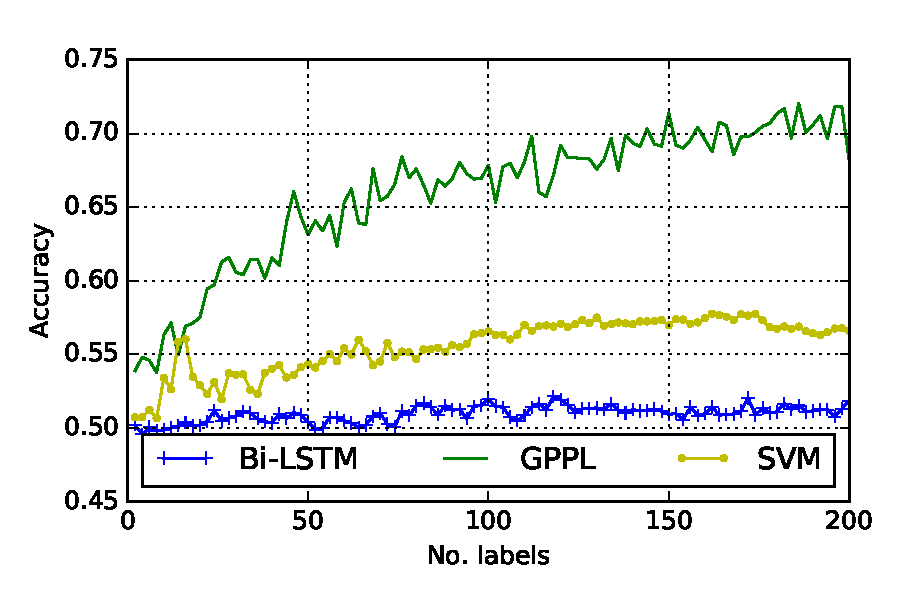
\includegraphics[width=1.0\columnwidth,trim=0 0 0 22,clip=true]{figures/active_learning/test_acc}
\caption{Active learning simulation for the three methods showing the mean accuracy of preference pair classifications over 32 runs.}
\label{fig:active_learning}
\end{figure}

% This plot is invalid because SVM and BLSTM are trained on the output from PageRank with all the data!
% \begin{figure}
% 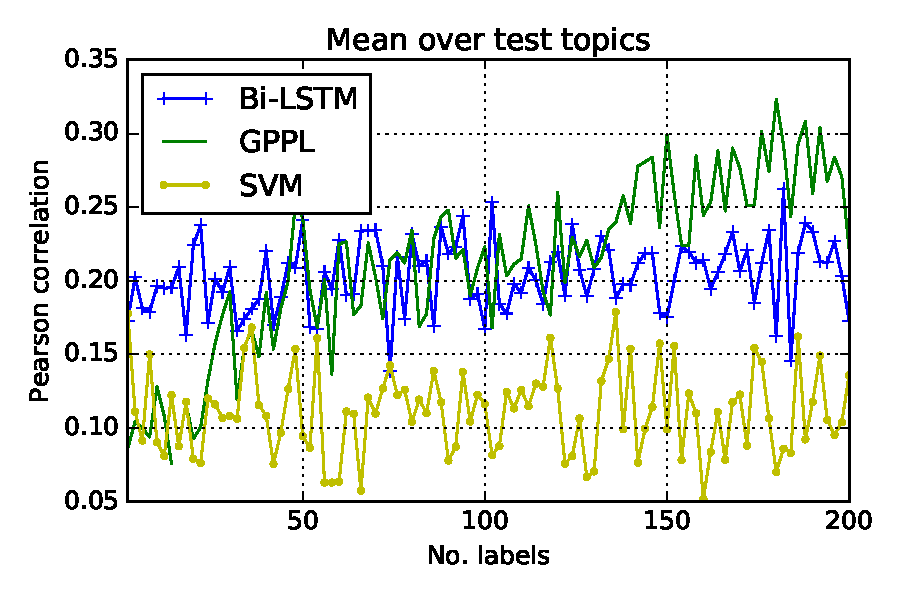
\includegraphics[width=1.0\columnwidth,trim=0 0 0 23,clip=true]{figures/active_learning/test_pearson}
% \caption{Active learning simulation for the three methods showing the mean pearson correlation with the gold standard ranking over 32 runs.}
% \end{figure}

\subsection{Experiment 5: Embeddings}

In our previous experiments, we found that including mean Glove word embeddings boosted performance above only using linguistic features. However, there are several alternative methods to mean word embeddings for representing longer pieces of text, 
notably skip-thoughts\cite{skipthoughts} and Siamese-CBOW\cite{siamesecbow}.
We compare mean Glove embeddings with skip-thoughts embeddings trained on the ... corpus\cite{skipthoughts_embeddings} and Siamese-CBOW embeddings trained on the ...
corpus\cite{siamesecbow_embeddings}. 
The results are shown in Table \ref{tab:embeddings} showing that the best performance
was obtained using mean Glove embeddings. 
Further work may be required to assess whether skip-thoughts and Siamese-CBOW 
can be improved if trained on different corpora, or whether the mean word embeddings
are simply more informative for predicting convincingness on our chosen dataset.
% with both median heuristic length-scale and optimized length-scale to ensure that %differences in performance are not caused by the heuristic failing with certain embedding %types. Result: awaiting optimized results, but non-optimized results show that word mean %was most effective.
%\end{enumerate}
% Could be merged into 2 and 3
\begin{table*}
  \begin{tabularx}{\textwidth}{ | l | X | X | X | X |  X |  X |  X | X | X |}
  \hline
 \multicolumn{7}{| l |}{UKPConvArgStrict} \\   \hline
       & \multicolumn{6}{ l |}{Median heuristic}                                     & \multicolumn{3}{l|}{Optimised} \\
       &Glove &Skip-thoughts &SCBOW &ling+ Glove &ling+ Skip-th. &ling+ SCBOW &ling+ Glove &ling+ Skip-th. & ling+ SCBOW \\ \hline
  \\ \hline
Acc.:  & 0.71 & 0.67         & 0.69  & 0.79       & 0.74               & 0.77        & 0.80       & 0.78 & 0.78 \\
AUC:   & 0.77 & 0.72         & 0.75  & 0.87       & 0.81               & 0.85        & 0.87       & 0.85 & 0.85\\
CEE:   & 1.12 & 1.11         & 1.22  & 0.47       & 0.80               & 0.52        & 0.51       & 0.51 & 0.50\\
\hline \multicolumn{7}{| l |}{UKPConvArgRank} \\   \hline
Pears.:& 0.33 & 0.30         & 0.29  & 0.45       & 0.34               & 0.39        &   0.44     & 0.34 & 0.40\\
Spear.:& 0.44 & 0.49         & 0.40  & 0.65       & 0.59               & 0.63        &    0.67    & 0.52 & 0.63\\
Kend.: & 0.31 & 0.36         & 0.28  & 0.49       & 0.43               & 0.47        &    0.50    & 0.37 & 0.47\\
\hline
  \end{tabularx}
  \caption{Comparison between different types of embeddings with GPPL}
  \label{tab:embeddings}
\end{table*}

\subsection{Experiment 6: Informative Features}

Finally, we show how the length-scales learned by optimising GPPL can be used to identify
informative sets of features. Since a larger length-scale causes greater smoothing, 
a very large length-scale implies that the value of that feature is irrelevant when predicting 
the function. In contrast, small length-scales indicate more informative features, since their
precise value affects the latent preference function.
Figure \ref{fig:boxplot} shows the distribution of optimised length-scales on one fold of UKPConvArgStrict. The values shown are ratios of the optimised value to the median heuristic. 
Due to the computation time required, our optimisation procedure was limited to $25$ function evaluations. The large number of values close to $1$ may be due to the L-BFGS-B
algorithm not being able to optimise all features in the available time, but 
it also suggests that other features with larger gradients were prioritised for optimisation,
and hence that the median heuristic was a reasonable estimate for these features. 
The length-scales for many dimensions of the mean word embeddings were increased,
giving ratios close to $4x$ the median heuristic, suggesting that these dimensions may be
only very weakly informative. Table \ref{tab:extreme_features} shows the largest
and smallest ratios for embeddings and linguistic features. The unigram "safety" has
a very high length-scale, suggesting it is not informative and may be discarded. 
It is possible that continuing the optimisation procedure for a larger number of steps would 
identify large length-scales for other features that may be discarded. However, caution is 
required to avoid overfitting to the training set during optimisation\cite{overfitting_ml2}.
\begin{figure*}
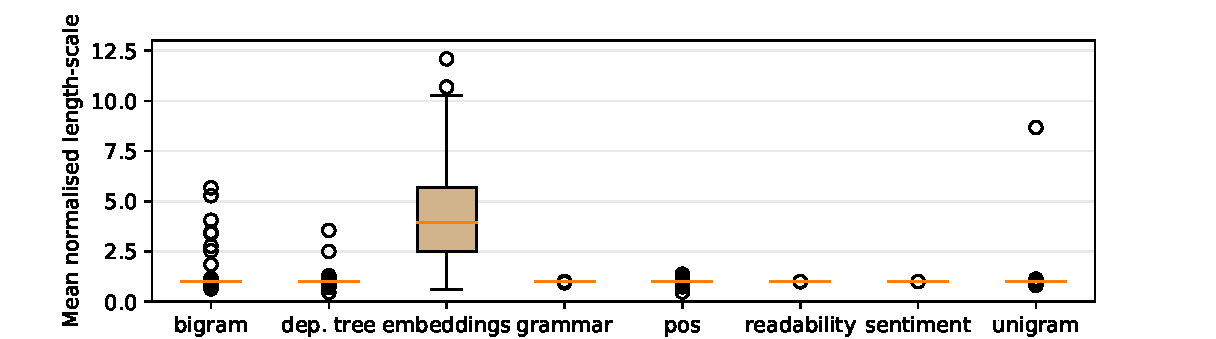
\includegraphics[width=\textwidth]{figures/features/boxplot}
\caption{Distribution of length-scales for each type of feature after optimisation. 
Values are relative to the median heuristic value before optimisation, optimised 
on fold "should physical education be mandatory in schools -- no", where 
optimisation increased accuracy from 75\% to 80\%. }
\label{fig:boxplot}
\end{figure*}
\begin{table}
  \begin{tabularx}{\columnwidth}{l | X }
  Feature & Ratio\\
  \hline
  ProductionRule-S-$>$ADVP,NP,VP,., & 0.466 \nonumber\\
  Pos-ngram-PP-O-CARD & 0.477 \nonumber\\
  Unigram-``safer", & 0.640 \nonumber\\
  \hline
  Bigram-``?"-``look" & 5.672 \nonumber\\
  Unigram-``safest" & 8.673 \nonumber\\
  Unigram-``safety" & 271.190 \nonumber\\
  \hline
  Embedding-dimension-19 & 0.610 \nonumber\\
  \hline
  Embedding-dimension-241 & 12.093 \nonumber\\
  \end{tabularx}
  \caption{Ratios of optimised to median heuristic length-scales: largest and smallest
  ratios for linguistic features and word embeddings.}
  \label{tab:extreme_features}
\end{table}
